\documentclass[12pt]{article}\usepackage[]{graphicx}\usepackage[]{color}
%% maxwidth is the original width if it is less than linewidth
%% otherwise use linewidth (to make sure the graphics do not exceed the margin)
\makeatletter
\def\maxwidth{ %
  \ifdim\Gin@nat@width>\linewidth
    \linewidth
  \else
    \Gin@nat@width
  \fi
}
\makeatother

\definecolor{fgcolor}{rgb}{0.345, 0.345, 0.345}
\newcommand{\hlnum}[1]{\textcolor[rgb]{0.686,0.059,0.569}{#1}}%
\newcommand{\hlstr}[1]{\textcolor[rgb]{0.192,0.494,0.8}{#1}}%
\newcommand{\hlcom}[1]{\textcolor[rgb]{0.678,0.584,0.686}{\textit{#1}}}%
\newcommand{\hlopt}[1]{\textcolor[rgb]{0,0,0}{#1}}%
\newcommand{\hlstd}[1]{\textcolor[rgb]{0.345,0.345,0.345}{#1}}%
\newcommand{\hlkwa}[1]{\textcolor[rgb]{0.161,0.373,0.58}{\textbf{#1}}}%
\newcommand{\hlkwb}[1]{\textcolor[rgb]{0.69,0.353,0.396}{#1}}%
\newcommand{\hlkwc}[1]{\textcolor[rgb]{0.333,0.667,0.333}{#1}}%
\newcommand{\hlkwd}[1]{\textcolor[rgb]{0.737,0.353,0.396}{\textbf{#1}}}%
\let\hlipl\hlkwb

\usepackage{framed}
\makeatletter
\newenvironment{kframe}{%
 \def\at@end@of@kframe{}%
 \ifinner\ifhmode%
  \def\at@end@of@kframe{\end{minipage}}%
  \begin{minipage}{\columnwidth}%
 \fi\fi%
 \def\FrameCommand##1{\hskip\@totalleftmargin \hskip-\fboxsep
 \colorbox{shadecolor}{##1}\hskip-\fboxsep
     % There is no \\@totalrightmargin, so:
     \hskip-\linewidth \hskip-\@totalleftmargin \hskip\columnwidth}%
 \MakeFramed {\advance\hsize-\width
   \@totalleftmargin\z@ \linewidth\hsize
   \@setminipage}}%
 {\par\unskip\endMakeFramed%
 \at@end@of@kframe}
\makeatother

\definecolor{shadecolor}{rgb}{.97, .97, .97}
\definecolor{messagecolor}{rgb}{0, 0, 0}
\definecolor{warningcolor}{rgb}{1, 0, 1}
\definecolor{errorcolor}{rgb}{1, 0, 0}
\newenvironment{knitrout}{}{} % an empty environment to be redefined in TeX

\usepackage{alltt}
\usepackage{amsmath}
\usepackage{graphicx}
\usepackage{natbib}
\usepackage{url} % not crucial - just used below for the URL 
\usepackage{multirow}
\usepackage{mathtools}
\usepackage{amsfonts}
\usepackage{rotating}
\usepackage{booktabs}
\usepackage{verbatim}
\usepackage{mathrsfs}
\usepackage{hyperref}
\usepackage{pdflscape}
\usepackage{caption}
\usepackage{tablefootnote}
\usepackage{verbatim}
\usepackage{setspace}
\usepackage[utf8]{inputenc}
\usepackage{authblk}
\usepackage{pdfpages}
\usepackage{fancyhdr}
%\pdfminorversion=4
% NOTE: To produce blinded version, replace "0" with "1" below.
\newcommand{\blind}{0}

% DON'T change margins - should be 1 inch all around.
\addtolength{\oddsidemargin}{-.5in}%
\addtolength{\evensidemargin}{-.5in}%
\addtolength{\textwidth}{1in}%
\addtolength{\textheight}{1.3in}%
\addtolength{\topmargin}{-.8in}%
\IfFileExists{upquote.sty}{\usepackage{upquote}}{}
\begin{document}

\def\spacingset#1{\renewcommand{\baselinestretch}%
{#1}\small\normalsize} \spacingset{1}


%%%%%%%%%%%%%%%%%%%%%%%%%%%%%%%%%%%%%%%%%%%%%%%%%%%%%%%%%%%%%%%%%%%%%%%%%%%%%%

\if0\blind
{
  \title{\bf A Projection Pursuit Forest Algorithm for Supervised Classification}
  \author{Natalia da Silva\hspace{.2cm}\\
    Instituto de Estadística (IESTA), Universidad de la República\\
    and \\
    Dianne Cook \\
    Department of Econometrics and Business Statistics, Monash University\\
    and Eun-Kyung Lee\\
    Department of Statistics,  Ewha Womans University }
  \maketitle
} \fi

\if1\blind
{
  \bigskip
  \bigskip
  \bigskip
  \begin{center}
    {\LARGE\bf Title}
\end{center}
  \medskip
} \fi

\bigskip
\begin{abstract}
This paper presents a new ensemble learning method for classification problems called projection pursuit random forest (PPF). PPF uses the \verb# PPtree#  algorithm introduced in \cite{lee2013pptree}. In PPF, trees are constructed by splitting on linear combinations of randomly chosen variables. Projection pursuit is used to choose a projection of the variables that best separates the classes. Utilizing linear combinations of variables to separate classes takes the correlation between variables into account which allows PPF to outperform a traditional random forest when separations between groups occurs in combinations of variables.

The method presented here can be used in multi-class problems and is implemented into an R~\citep{RCore} package, \verb# PPforest#, which is available on CRAN.

\end{abstract}

\noindent%
{\it Keywords:} data mining, ensemble model, statistical computing, exploratory data analysis, high dimensional data
\vfill

\newpage
\spacingset{1.5} % DON'T change the spacing!
\section{Introduction}
\label{sec:intro}

There are two main features from a random forest algorithm~\citep{breiman2001random} that are broadly applicable for building ensemble classifiers from any basic method: bootstrap aggregation (bagging) and random predictor selection. Bagging stabilizes the variance~\citep{breiman1996bagging, breiman1996heuristics} and random predictor selection reduces correlation~ \citep{amit1997shape, ho1998random} between trees in the forest (ensemble components).

This paper presents the projection pursuit random forest (PPF), a new ensemble learning method for classification problems, built from trees utilizing combinations of predictors. PPF builds a forest from many projection pursuit trees (PPtree)~\citep{lee2013pptree}, which is available in the R package \verb# PPtreeViz#~\citep{PPtreeViz}. Projection pursuit~\citep{friedman1973projection} is used to find the linear combination of variables that best separates groups, and many different rules to make the actual split are provided.

Trees that use linear combinations of predictors in a split are known in the literature as oblique trees~\citep{kim2001,brodley,tan2005mml,truong2009fast,lee2013pptree}.
All these algorithms use different approaches for finding linear combinations of predictors upon which to make a split. Some of the methods used for selecting the linear combination include random coefficient generation, linear discriminant analysis, and linear support vector machines. Theoretically, these could also be used as a base underlying PPF.

In the machine learning literature numerous work has been conducted on algorithms for building forests from oblique trees~\citep{tan2006decision, menze2011oblique, do2010classifying}. The performance is reported to be better than random forests. A limitation of building on these approaches is the lack of readily available software.

In a PPF, for each split, a random sample of predictors is selected, an optimal linear combination for separating the classes is computed by using projection pursuit. The algorithm is targeted for problems where classes can be separated by linear combinations of predictors, which define separating hyperplanes that are oblique to the axes rather than orthogonal to them. This may sound like a support vector machine~\citep{Cortes1995}, but the tree construction makes it different -- the separation in linear combinations is examined for subspaces of the high-dimensional space.  PPF also accommodates imbalanced classes by using stratified bootstrap samples, and variable importance measures are computed using the coefficients of the projections. PPF can be used for multi-class problems and is implemented into an R package, called \verb# PPforest#.

PPF can outperform RF, and an application is included to demonstrate this. However, it has the same interpretability and diagnostics as RF, which helps analysts to better understand the data.

This paper is organized as follows. Section \ref{PPT} explains PPtree algorithm underlying PPF. Section \ref{PPFsec} describes the PPF algorithm; diagnostics, including how to compute variable importance and the implementation details. Section \ref{perfsec} evaluates the algorithm performance on benchmark machine learning data in comparison with other tree methods. Section \ref{options} explains the diagnostics in comparison to those from RF, and discusses parameter selection. An application illustrating the power of PPF over other tree methods is provided in Section \ref{rnaapli}. Section \ref{discpp1} discusses possible extensions and future directions.

\section{Background on the projection pursuit tree}
\label{PPT}





The projection pursuit algorithm searches for low dimensional projections that optimize a function which measures some aspect of interest, for PPtree, this is class separation. \cite{friedman1973projection} coined the term ``projection pursuit'', but the ideas existed earlier than this, and are discussed in~\cite{kruskal1969toward}. Indexes for finding projections that separate classes were developed in~\cite{lee2005projection} (LDA) and~\cite{lee2010projection} (PDA). These form the basis of PPtree, and are explained below.

Let $\mathbf{x}_{gi}$ be a $p$-dimensional data vector, representing the $i^{th}$ observation of the $g^{th}$ class, with $g = 1,\ldots, G$, $G$ is the number of classes, $i = 1,\ldots , n_g$, and $n_g$ is the number of observations in class $g$. The LDA index is defined as follows:

\begin{equation}
 I_{LDA}(A) = \left\{
  \begin{array}{l l}
    1-\frac{|A^T WA|}{|A^T(W+B)A|} &  \text{for}~|A^T(W+B)A|\neq 0\\
    0 &  \text{for}~|A^T(W+B)A|= 0
  \end{array} \right.
  \end{equation}

\noindent where $p\times k$ matrix $A = [a_1, a_2 , . . . , a_k ]$ defines an orthonormal projection from $p$-dimensions onto a $k$-dimensional subspace, 
$B=\sum_{g=1}^G n_g(\bar{\mathbf{x}}_{g.}-\bar{\mathbf{x}}_{..})(\bar{\mathbf{x}}_{g.}-\bar{\mathbf{x}}_{..})^{T}$ is the between-group sum of squares, and 
$W=\sum_{g=1}^{G}\sum_{i=1}^{n_g}(\mathbf{x}_{gi}-\bar{\mathbf{x}}_{g.})(\mathbf{x}_{gi}-\bar{\mathbf{x}}_{.g})^T$ is the within-group sum of squares. If the LDA index value is high, there is a large difference between classes.

 
\begin{figure}[!t]
\begin{knitrout}
\definecolor{shadecolor}{rgb}{0.969, 0.969, 0.969}\color{fgcolor}
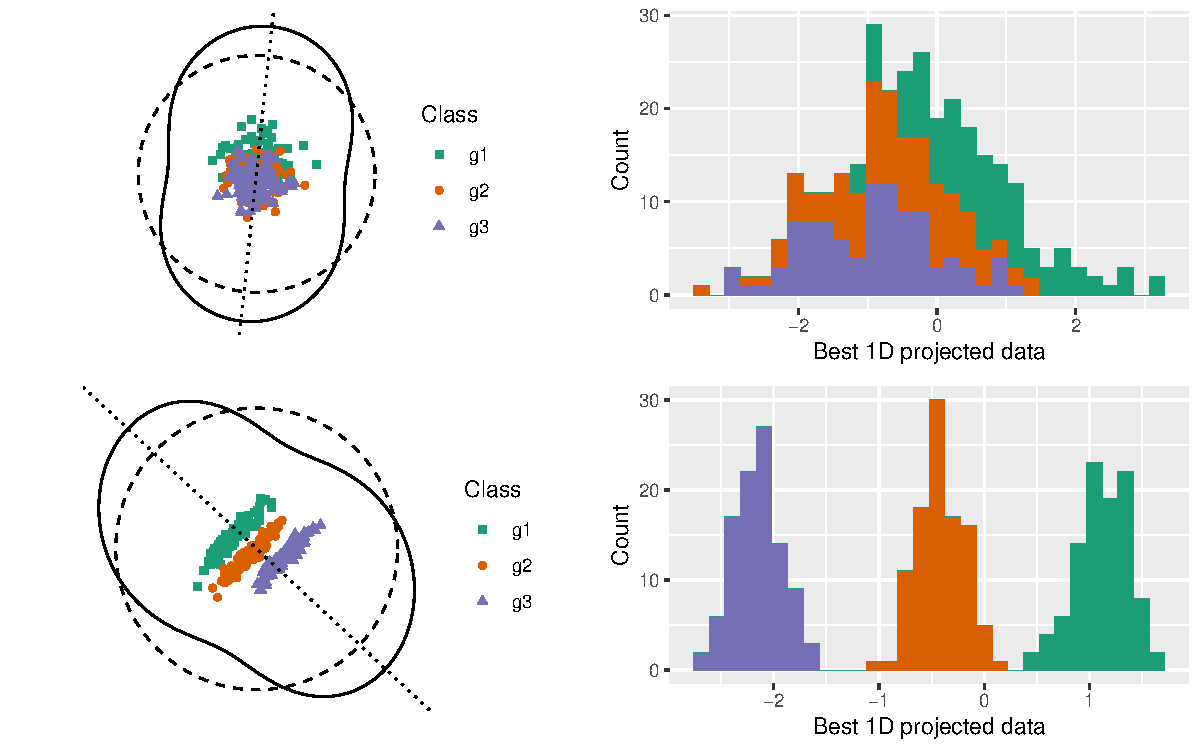
\includegraphics[width=\maxwidth]{figure/huber-1} 

\end{knitrout}
\caption{Behavior of the LDA index on 1D projections shown using a Huber plot for simulated data, two different sets of 2D. The solid line indicates index value for each 1D projection of the 2D data. The dashed circle indicates the median index value across all projections, and the dotted line corresponds to the projection producing the maximum index value. The histogram shows the projected data corresponding the maximum index value. \label{huberpl}}
\end{figure}

Figure \ref{huberpl} examines the behavior of the LDA index on two 2D simulated data sets, using Huber's plot~\citep{huber1990data} available in the \texttt{PPtreeViz} package~\citep{PPtreeViz}. This plot shows the projection pursuit index values in all possible directions in a 2D space. These indices are calculated using the projections for ($cos \theta$, $sin \theta$), $\theta$ = $1^{\circ}$, . . . , $180^{\circ}$. For each projection, the index value is computed on the projected data, and displayed as the solid line. The circle (dashed line) is a guideline, and corresponds to the median of all index values, with the solid line. The projection corresponding to the maximum index value is indicated as a dotted line, and the projected data is shown in the histogram. 
 
The PDA index is useful when $n\leq p$ and when the variables are highly correlated. In these situations the maximum likelihood variance-covariance matrix estimator will be close to singular, affecting the inverse calculation. The PDA index adjusts the variance-covariance matrix calculation, as follows:

\begin{equation}
I_{PDA}(A,\lambda)=1-\frac{|A^T W_{PDA}A|}{|A^T (W_{PDA}+B) A|}
\end{equation}

\noindent where notation as for the LDA index, with the addition of $\lambda \in [0,1)$ is a shrinkage parameter, and a different within group sum of squares, $W_{PDA}(\lambda)=\mbox{diag}(W)+(1-\lambda)\mbox{offdiag}(W)$.


\begin{figure}[!t]
\begin{knitrout}
\definecolor{shadecolor}{rgb}{0.969, 0.969, 0.969}\color{fgcolor}
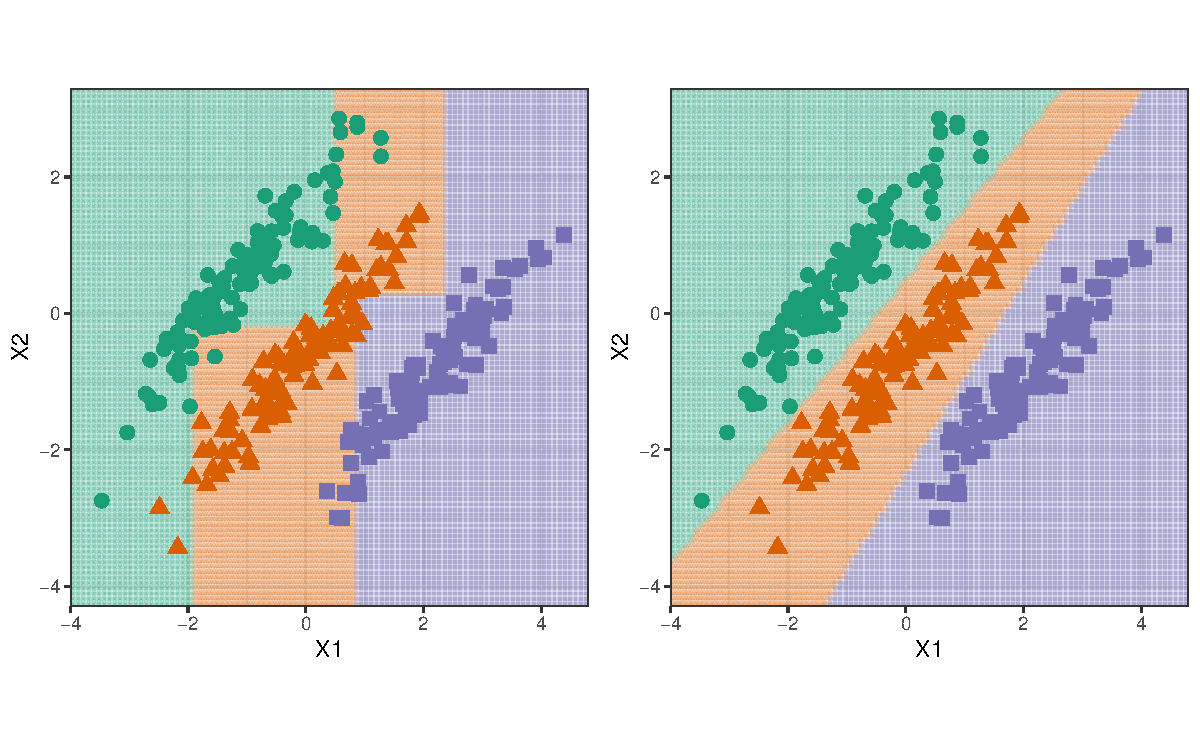
\includegraphics[width=\maxwidth]{figure/boundss-1} 

\end{knitrout}
 \vspace*{-0.3cm}
 \caption{Comparison of decision boundaries for the  \texttt{rpart} (left) and PPtree (right) algorithms on 2D simulated data. The partitions generated by PPtree algorithm are oblique to the axis, incorporating the association between the two variables.\label{bounds}}
\end{figure}


The PPtree algorithm uses a multi-step approach to fit a multi-class model by finding linear combinations to split on. Figure \ref{bounds} compares the boundaries that would result from a classification tree fitted using the rpart algorithm~\citep{therneau2010rpart} and the PPtree algorithm.

Figure \ref{diagpp1} illustrates the PPtree algorithm for three classes, and the algorithm steps are detailed below. Let  $d_n =\{(\mathbf{x_i},y_i)\}_{i=1}^n$ be the data set where $\mathbf{x_i}$ is a  p-dimensional vector of explanatory variables and  $y_i\in \mathscr{G}$ ($\mathscr{G} =\{1,2,\ldots G\}$) represents class information with $i=1,\ldots n$.

\begin{enumerate}
\item Optimize a projection pursuit index to find an optimal one-dimensional projection, $\alpha^*$, for separating all classes in the current data yielding projected data $z = \alpha^*x$.
\item On the projected data, $z$, redefine the problem into a two class problem using the distances among the means of classes, and assign a new label, either $g_1^*$ or $g_2^*$ to each observation, generating a new class variable $y_i^*$. Note that this requires joining two or more groups into one, so that the new groups $g_1^*$ and $g_2^*$ possibly contain more than one of the original classes. 

\item Find an optimal one-dimensional projection $\alpha^{**}$, using $\{(\mathbf{x_i},y_i^*)\}_{i=1}^n$ to separate the two class problem $g_1^*$ and $g_2^*$. The best separation of $g_1^*$ and $g_2^*$ is determined in this step providing the decision rule for the node,

\begin{quote}
if $\alpha^{**T}M_1< c$ then assign $g_1^*$ to the left node else assign $g_2^*$ to the right node,
\end{quote}
\noindent where $M_1$ is the mean of $g_1^*$.
\item For each group, all the previous steps are repeated until $g_1^*$ and $g_2^*$ have only one class from the original classes. The depth of PPtree is at most the number of classes.
\end{enumerate}

\begin{figure}[!hbt]
\centering
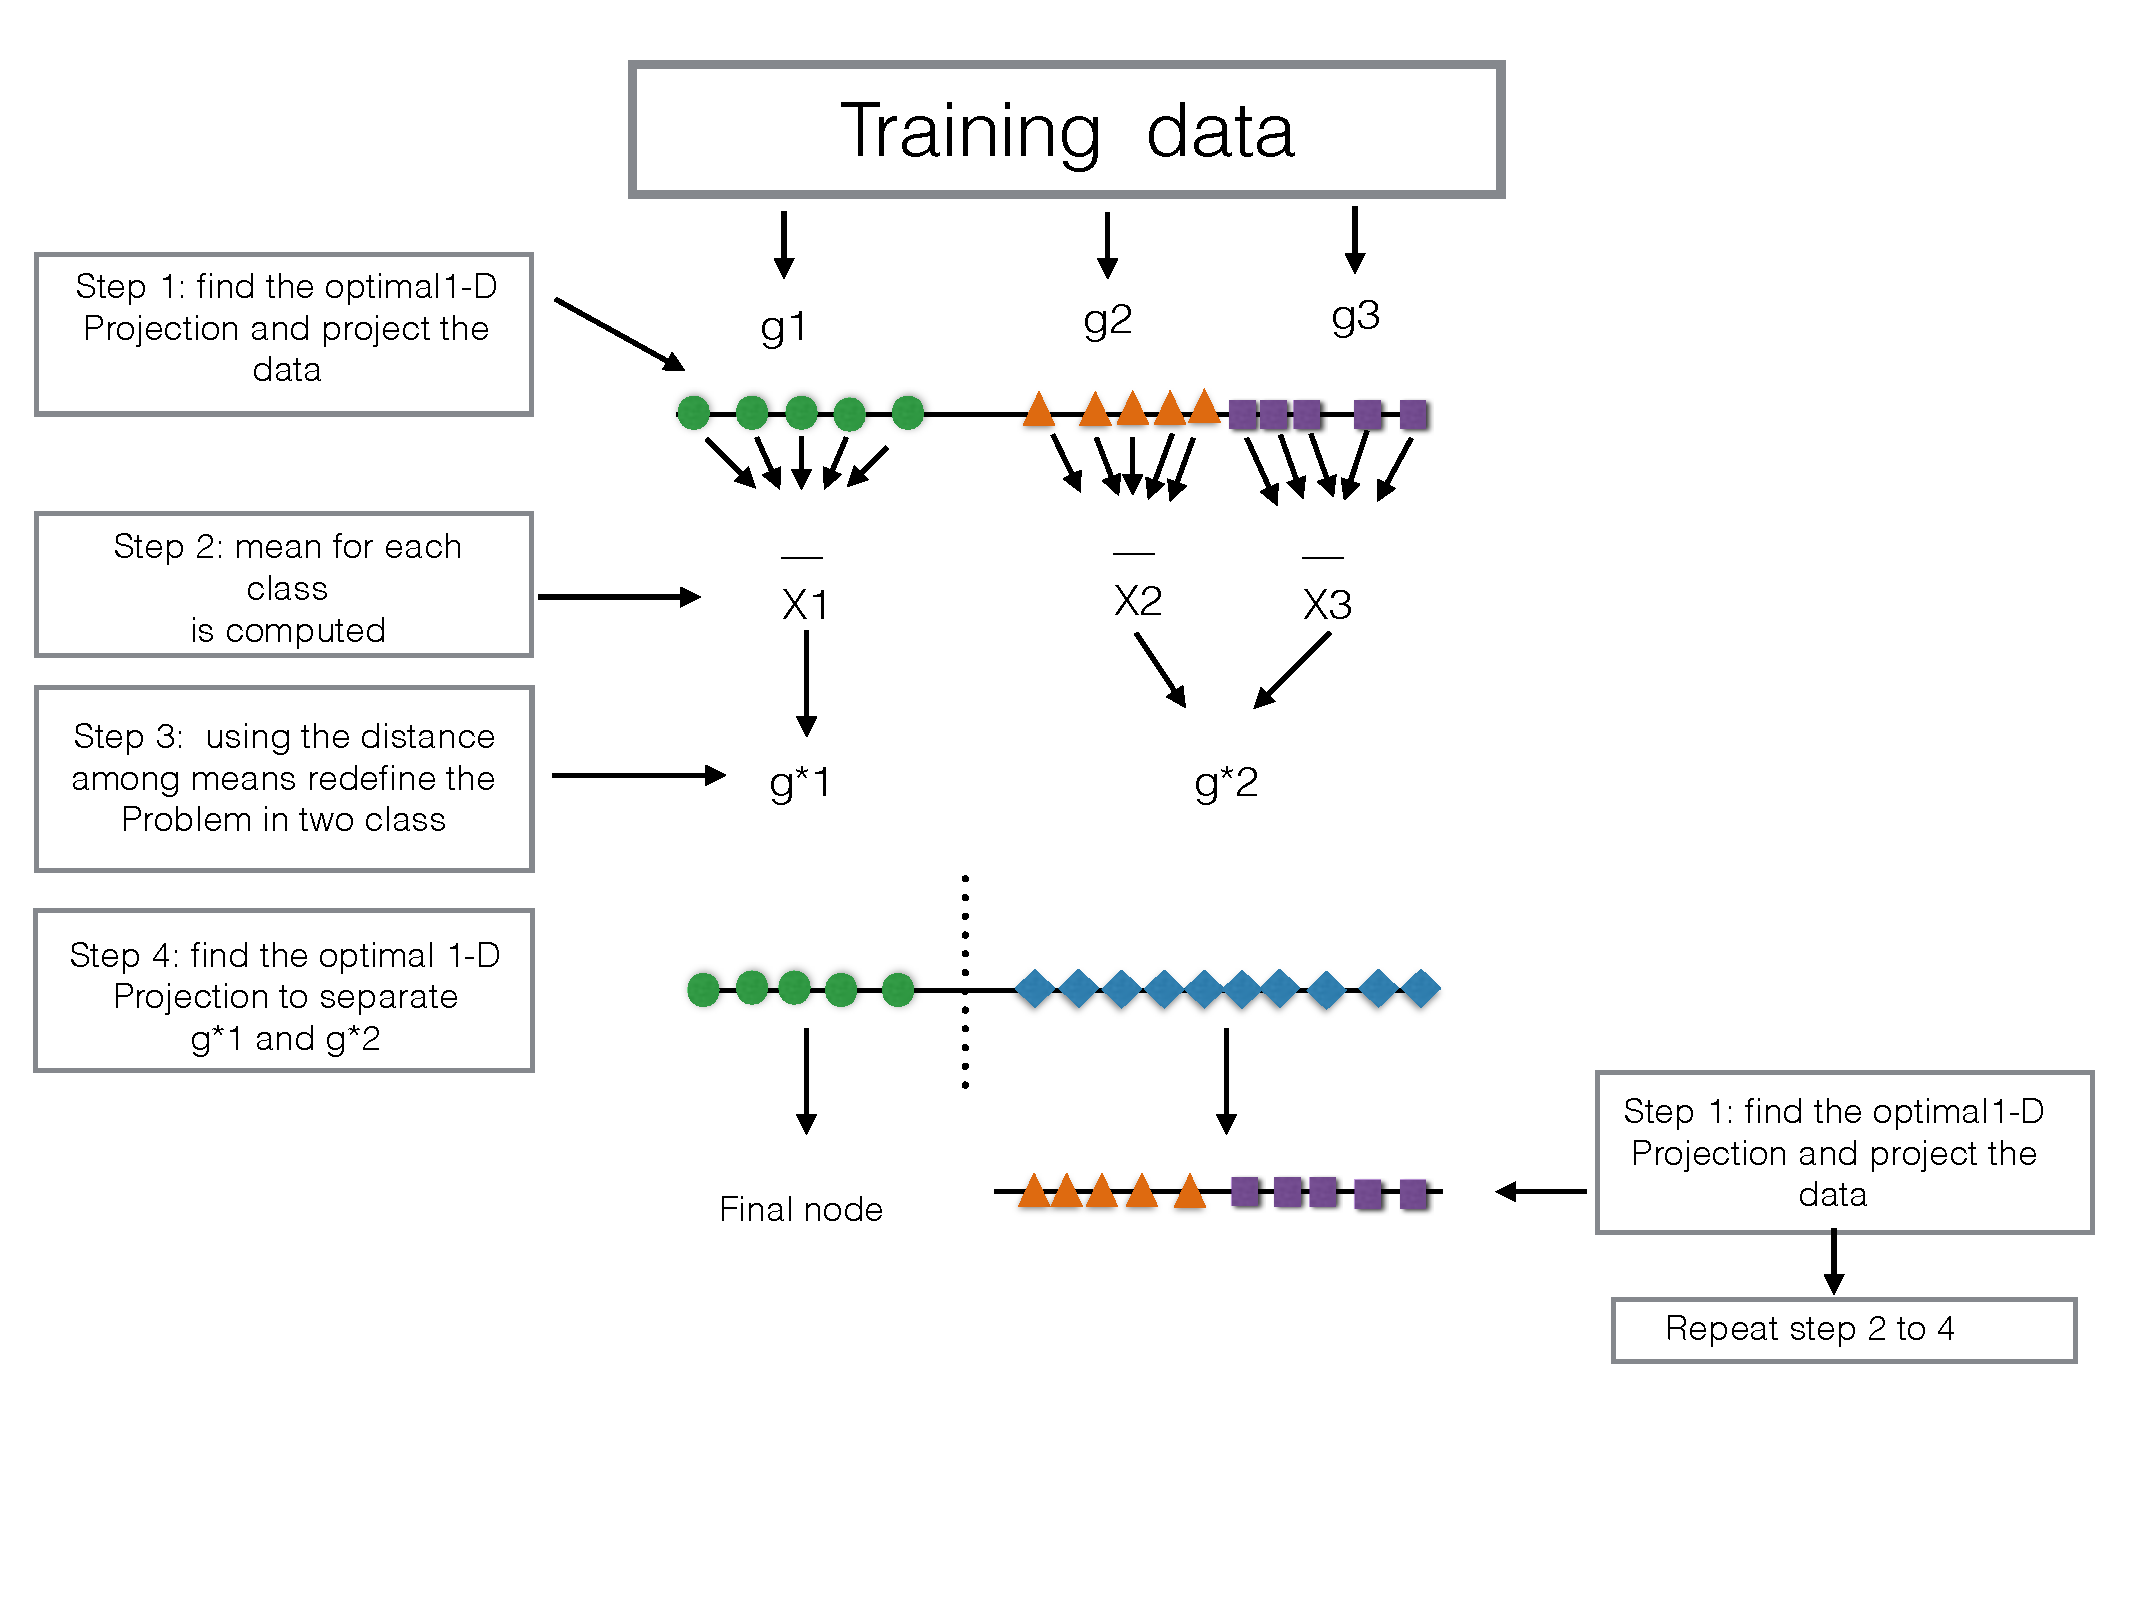
\includegraphics[width=1\linewidth]{diag2.pdf}

\caption{Illustration of the PPtree algorithm for $g=3$ classes. It is a dual pass algorithm for multiclass problems, for each split. It first finds the best separation and combines classes into two super-groups. It then searches again for the best separation between these two super-groups and splits on this. It proceeds sequentially on the subsets in the nodes, but only $g-1$ splits are allowed. \label{diagpp1}}
\end{figure}

\newpage

\section{Projection pursuit random forest}\label{PPFsec}


This section provides the definition of PPF for classification, an explanation of the algorithm, implementation details, and a description of how the diagnostics are defined and computed. 

\subsection{Definition}

This definition follows closely the original random forest notation in \cite{breiman2001random}, a more recent overview paper by \cite{Biau:2008}, and is important to provide here for consistency in the PPF explanation. Let the random vector of predictor variables $\mathbf{X}\in \Re^p$  and  the output random variable $Y \in \mathscr{G}$, where $\mathscr{G}$ is a finite set such that $\mathscr{G}=\{1,2, \ldots, G\}$. The training sample is defined as $D_n=\{(\mathbf{X_1}, Y_1), \ldots (\mathbf{X}_n, Y_n)\}$ of i.i.d $\Re^p \times \mathscr{G}$ random variables $(p\geq 2)$.
The objective is to build a classifier which predicts $y$ from $\mathbf{x}$ using $D_n$ given an ensemble of classifiers $h$.

 A projection pursuit classification random forest can be defined as a collection of randomized classification trees $\{h_n(\mathbf{x}, \Theta_m, D_n), m\geq 1\}$  where $\{\Theta_m\}$ are i.i.d.~random vectors. $\Theta_m$ includes the two sources of randomness in the tree (random variable selection and random bootstrap sample), then $\Theta_m$ has information about which variables were selected in each partition and which cases were selected in the bootstrap sample.

For each tree, $h_n$, a unique vote is collected based on the most popular class for the selected predictor variables.  Equation \ref{rfesti} defines the PPF estimator based on combining the trees.

\begin{eqnarray}\label{rfesti}
f_n(\mathbf{X}, D_n )&=& \operatorname*{arg\,max}_{g\in \mathscr{G}} \{E_{\Theta}(I[h_n(\mathbf{X}, \Theta, D_n)=g])\}\\ \nonumber
&=& \operatorname*{arg\,max}_{g\in \mathscr{G}} P_{\Theta}(h_n(\mathbf{X}, \Theta, D_n)=g)
\end{eqnarray}

\noindent $E_{\Theta}$ is the expectation wrt $\Theta$, conditionally on $\mathbf{X}$ and $D_n$.
In practice, the PPF estimator is evaluated by generating $B$ random trees and take the average of the individual outcomes. This procedure is justified in a similar way to the original random forest defined by \cite{breiman2001random}, and is based on the Law of the Large Numbers~\citep{athreya2006measure}.

Equation \ref{predfor} describes the prediction of a new observation $\mathbf{x_0}$.

\begin{equation}
\hat f_n(\mathbf{x_0})= \operatorname*{arg\,max}_{g\in \mathscr{G}} \sum_{k=1}^B I [ h_n (\mathbf{x_0}, \Theta_{bk} )= g]
\label{predfor}
\end{equation}

\subsection{Algorithm }

\begin{enumerate}

\item Let $n=\sum_{i=1}^G n_i$ the total number of cases in the training set $d_n=\{\mathbf{x_i}, y_i\}_{i=1}^n$. $B$ stratified bootstrap samples from $d_n$ are taken. Then for each class, independently and uniformly re-sample cases from $d_{ng}$ (training data set for group $g$) with size $n_g$ to create a stratified bootstrap data set  $\{bk= b_{k1}, b_{k2}, \ldots b_{kg}\}$.

\item Use a bootstrap sample $bk$ to grow a PPtree $(h_n(\mathbf{x}, \Theta_{bk}))$ to the largest extent possible without pruning. (Note that the depth of the PPtree is at most $G-1$, where $G$ is the number of classes).

\begin{enumerate}
\item Start with all the cases in $b_k$ in the root node.
\item A simple random sample of $m$ predictor variables from the set of all the predictor variables $M$ is drawn, where $m<<M$.
\item Find the optimal one-dimensional projection $\alpha^*$ to separate all the classes in $b_k$.
\item If more than two class, then reduce the number of classes to two by comparing means, and assign new labels, $g_1^*$ and $g_2^*$ to each case (called the new response $y_i^*$ in $b_k$).

\item Find the optimal one-dimensional projection, $\alpha^{**}$, using the bootstrap data set with the relabeled response, $y^*$, to separate $g_1^*$ and $g_2^*$.
The linear combination is computed by optimizing a projection pursuit index to get a projection of the variables that best separates the classes using the $m$ random selected variables. Two index options are available LDA or PDA.
\item Compute the decision boundary $c$.
Eight different rules to define the cutoff value of each node can be used. All the rules are defined in \cite{PPtreeViz}.
\item Keep $\alpha^{**}$ and $c$.
\item Separate the data into two groups using the new labels $g_1^*$ and $g_2^*$.
\item Repeat from (b) to (h) if $g_1^*$ or $g_2^*$ have more than two original classes.
\end{enumerate}
\item Repeat 2 for $k = 1,\ldots B$.
\item The output is the ensemble of PPtrees, $\{h_n^{bk}\}_{k=1}^B$.
\end{enumerate}

Split values on the projected data can be computed by one of eight methods, which use the group means, or medians, sample size and variance or IQR weighting

Figure \ref{diagppf} has a diagram illustrating the PPforest algorithm.

\begin{figure}[!ht]
\centering
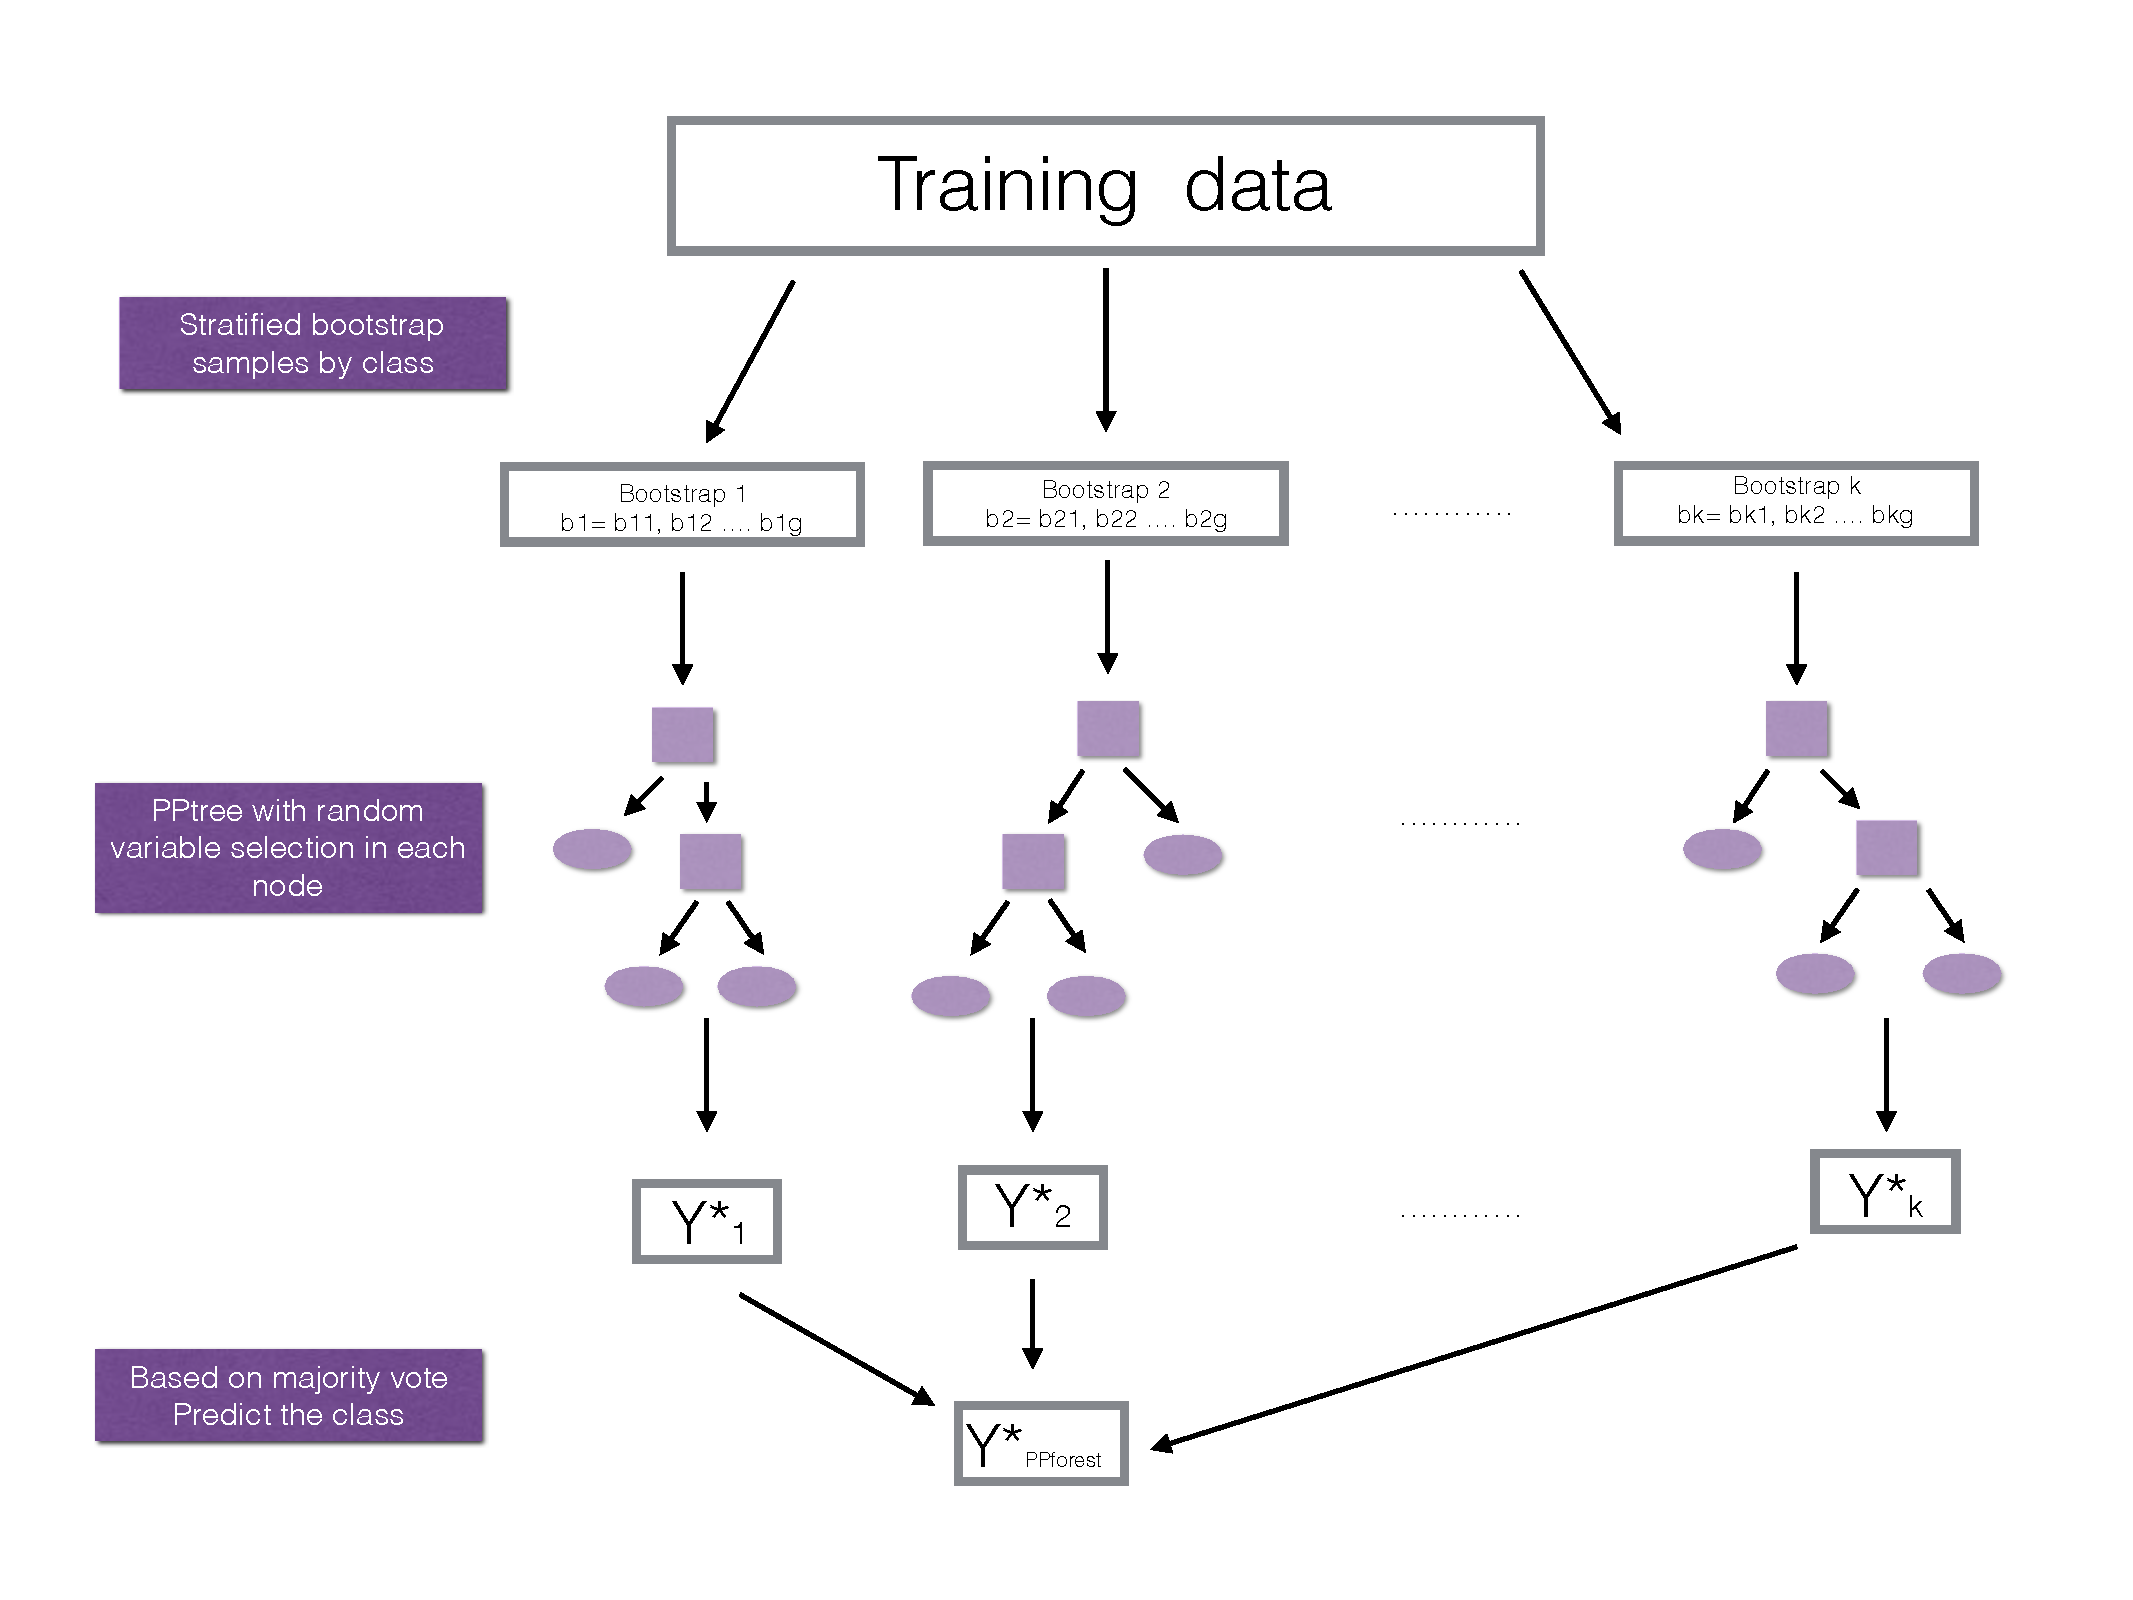
\includegraphics[width=1\linewidth]{diagram.pdf}
 \vspace*{-0.5cm}
\caption{Illustration of the PPforest algorithm. It is effectively the same as a random forest algorithm except that the PPtree classifier is used on each bootstrap sample. \label{diagppf}}
\end{figure}

\subsection{Implementation}
\label{impl}

The R package \verb# PPforest#~\citep{PPforestpkg}, provides an implementation of PPF. (The development version is available at \url{https://github.com/natydasilva/PPforest}.) 
The initial code for PPforest was developed entirely in R. It was subsequently profiled using \verb# profvis#~\citep{profvis}, and two code optimization strategies were employed: translate main functions into \verb# Rcpp#~\citep{eddelbuettel2011rcpp} and parallelization  using \verb# plyr#. The \verb# microbenchmark# package was used to compare the speed before and after optimization, and also for the comparison in Figure \ref{ratiotim} which shows the performance for a range of sample size ($n$), dimension ($p$), groups ($g$), number of trees ($m$) and proportion of variables considered at each node. The proportion has the largest effect on speed.

\begin{figure}[!ht]
\begin{knitrout}
\definecolor{shadecolor}{rgb}{0.969, 0.969, 0.969}\color{fgcolor}
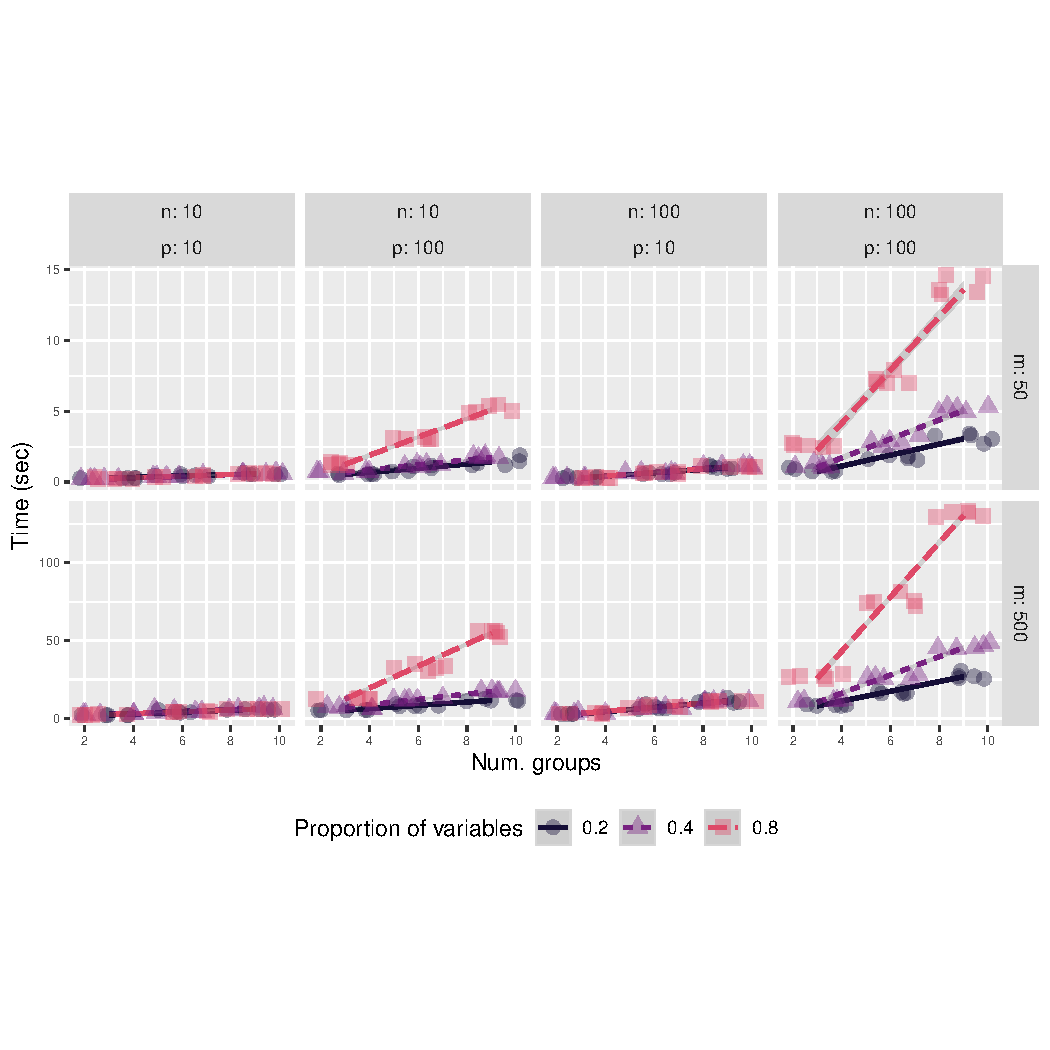
\includegraphics[width=15cm,height=15cm]{figure/resus-1} 

\end{knitrout}
\vspace{-3cm}
\caption{Computational performance for different sample size ($n$), number of variables ($p$), number of groups ($g$), number of trees ($m$) and proportion of variables considered for each node. Computational speed suffers most when the proportion of variables is high.\label{ratiotim}}
\end{figure}

\subsection{PPF diagnostics}

The process of bagging and combining results from multiple trees produces numerous diagnostics which can provide a lot of insight into the class structure in high dimensions. Because ensemble methods are composed of many models fitted to subsets of the data, many statistics can be calculated to be analyzed as a separate data set. This provides the ability to understand how the model is working. The diagnostics of interest are the error rate, variable importance measure, vote matrix, and proximity matrix. 
These diagnostics are used to assess model complexity, individual model contributions, variable importance and dimension reduction, and uncertainty in prediction associated with individual observations. Most of the diagnostics work as in RF, with the exception being the variable importance measure, which is specific to PPforest.


\subsubsection{Model error}

Using the out-of-bag (oob) cases from bagged trees in the forest construction allows ongoing estimates of the generalization error for an ensemble of trees, described in \cite{breiman2001random}.
Given a training data set $d_n$, $B$ bootstrap samples from $d_n$ are taken. For each bootstrap sample ($b= 1, 2, \ldots B$), a \verb# PPtree# classifier $h_n(\mathbf{x}, \Theta_b)$ is constructed, and a majority vote is used to get the PPF predictor.
The oob cases are used to get the error rate estimates. For each $\{\mathbf{x_i}, y_i\}$ in $d_n$, the votes are aggregated only for the classifiers $h_n(\mathbf{x}, \Theta_b)$ that do not contain $\{\mathbf{x_i}, y_i\}$. Hence, PPF is called the out-of-bag classifier, and the error rate for this classifier (out-of-bag error rate) is the estimate of the generalized error. The out-of-bag error rate is a measure for each model that is combined in the ensemble and is used to provide the overall error of the ensemble.

\subsubsection{Variable importance}

PPF calculates variable importance in two ways: (1) permuted importance using accuracy,  and (2) importance based on projection coefficients on standardized variables.
The permuted variable importance is comparable to the measure defined in the classical random forest algorithm. It is computed using the oob cases for the tree $k\;\;(B^{(k)})$ for each $X_j$ predictor variable.  Then the
permuted importance of the variable $X_j$ in the tree $k$ can be defined as:

\[
IMP^{(k)}(X_j) = \frac{\sum_{i \in B^{(k)} } I(y_i=\hat y_i^{(k)})-I(y_i=\hat y_{i,P_j}^{(k)})}{|B^{(k)}|}
\]

\noindent where $\hat y_i^{(k)}$%=h(x_i,\Theta_k)$
 is the predicted class for the observation $i$ in the tree $k$, and $y_{i,P_j}^{(k)}$ is the predicted class for the observation $i$ in the tree $k$ after permuting the values for variable $X_j$. The global permuted importance measure is the average importance over all the trees in the forest.
 
This measure is based on comparing the accuracy of classifying oob observations using the true class with permuted (nonsense) class.

For the second importance measure, the coefficients of each projection are examined. The magnitude of these values indicates importance if the variables have been standardized. The variable importance for a single tree is computed by a weighted sum of the absolute values of the coefficients across node, then the weights take the number of classes in each node into account($cl_{nd}$)~\citep{lee2013pptree} .
The importance of the variable $X_j$ in the PPtree $k$ can be defined as:

\[
IMP_{pptree}^{(k)}(X_j)=\sum_{nd = 1}^{nn}\frac{|\alpha_{nd}^{(k)}|}{cl_{nd} }
\]

\noindent where $\alpha_{nd}^{(k)}$ is the projected coefficient for node $ns$ and variable $k$ and $nn$ the total number of node partitions in the tree $k$.

The global variable importance in a PPforest then can be defined in different ways. The most intuitive are the average variable importance from each PPtree across all the trees in the forest.
\[
IMP_{ppforest1}(X_j)=\frac{\sum_{k=1}^K IMP_{pptree}^{(k)}(X_j)}{K}
\]
Alternatively, a global importance measure is defined for the forest as a weighted mean of the absolute value of the projection coefficients across all nodes in every tree. The weights are based on the projection pursuit indexes in each node ($Ix_{nd}$), and 1-(OOB-error of each tree)($acc_k$).

\[IMP_{ppforest2}(X_j)=\frac{\sum_{k=1}^K acc_k \sum_{nd = 1}^{nn}\frac{Ix_{nd}|\alpha_{nd}^{(k)}|}{nn }}{K}
\]

\subsubsection{Observational level diagnostics}

The vote matrix is an uncertainty measure for each observation, across models, is the proportion of times that a case is predicted to be in each class. If a case is always predicted to be the one class, there is no uncertainty about its group, and if this matches the true class then it is correctly labeled. Cases that are predicted to be multiple classes, indicate difficult-to-classify observations. These cases may be important in that they might indicate special attention is needed in some neighborhoods of the data space, or more simply, could be errors in measurements in the data.

In a tree, each pair of observations can be in the same terminal node or not. Tallying this up across all trees in a forest gives the proximity matrix, an $n\times n$ matrix of the proportion of trees that the pair shares a terminal node. A proximity matrix can be considered to be a similarity matrix. This is typically used for follow-up cluster analysis to assess the strength of the class structure, and whether there are additional unlabeled clusters.

\section{Performance comparison}\label{perfsec} 

This section presents simulation results and a benchmark data study to examine the predictive performance of PPF in comparison to other methods. In the benchmark data study, PPF is compared with PPtree, CART and RF. The simulation results are designed to compare PPF with RF on data with linear projections defining class differences.

The performance of PPF is compared with the classification methods, PPtree, CART and RF using 10 benchmark data sets taken from the UCI Machine Learning archive \citep{Lichman}. Table \ref{bench.tab} presents summary information about the benchmark data, number of groups, cases, and predictors for each data set. The \textit{imbalance} between groups is measured by the range of group size proportions and \textit{correlation} is the average of all pairwise correlation coefficients among predictor variables.

% latex table generated in R 3.5.2 by xtable 1.8-2 package
% Sun Sep  8 06:41:16 2019
\begin{table}[ht]
\centering
\caption{Overview of benchmark data: number of cases, predictors, groups, imbalance and correlation. Imbalance indicates relative class sizes (0=balanced classes), and higher correlation indicates the potential for separations occurring in combinations of variables.} 
\label{bench.tab}
\begin{tabular}{lrrrrr}
  \hline
Data & Cases & Predictors & Groups & Imbalance & Correlation \\ 
  \hline
crab & 200 &   5 &   4 & 0.00 & 0.95 \\ 
  lymphoma &  80 &  50 &   3 & 0.41 & 0.75 \\ 
  NCI60 &  61 &  30 &   8 & 0.07 & 0.56 \\ 
  parkinson & 195 &  22 &   2 & 0.51 & 0.50 \\ 
  fishcatch & 159 &   6 &   7 & 0.31 & 0.46 \\ 
  leukemia &  72 &  40 &   3 & 0.40 & 0.44 \\ 
  olive & 572 &   8 &   9 & 0.32 & 0.35 \\ 
  wine & 178 &  13 &   3 & 0.13 & 0.30 \\ 
  image & 2310 &  18 &   7 & 0.00 & 0.28 \\ 
  glass & 214 &   9 &   6 & 0.31 & 0.23 \\ 
   \hline
\end{tabular}
\end{table}


For each benchmark data set, $2/3$ of the observations are randomly chosen and used for training while the remaining $1/3$ are used as test data for computing predictive error. This procedure is repeated 200 times and the mean error rate is reported in Table \ref{res}. In PPF, the number of variables selected in each node partition is a tuning parameter, the proportion of variables selected at each partition. Three different values were used (0.6, 0.9 and the RF default). The test error reported for PPF is the best from these.

The results show that PPF has a better performance in the test data set than the other methods for the crab, fishcatch, leukemia, lymphoma, olive and wine data, while the RF test error is smaller for glass, image, NCI60 and parkinson data. When there is a big improvement over RF, PPtree also performs well, and the reason is that the difference between classes is in combinations of variables so using linear combinations provides better performance. PPF has the advantage, over PPtree, of providing additional diagnostics for a problem, so even though performance is similar, the diagnostics obtained are beneficial. Overall, PPF performs comparably to these other tree-based methods, and provides consistently low error rates.

% latex table generated in R 3.5.2 by xtable 1.8-2 package
% Sun Sep  8 06:41:16 2019
\begin{table}[ht]
\centering
\caption{Comparison of  CART, PPtree, RF and PPF results with various data sets. The mean of training and test error rates from 200 re-samples is shown. (Order of rows is same as in Table \ref{bench.tab}.) PPF performs favorably compared to the other methods. \label{res}} 
\begin{tabular}{l||cccc||cccc}
  \hline\hline &  \multicolumn{4}{c||}{TRAINING} & \multicolumn{4}{c}{TEST} \\ \hline
Data & CART & PPtree & RF & PPforest & CART & PPtree & RF & PPforest \\ 
  \hline
crab & 0.277 & 0.044 & 0.244 & 0.046 & 0.453 & 0.057 & 0.238 & 0.057 \\ 
  lymphoma & 0.052 & 0.000 & 0.100 & 0.000 & 0.155 & 0.069 & 0.081 & 0.053 \\ 
  NCI60 & 0.503 & 0.000 & 0.458 & 0.019 & 0.676 & 0.423 & 0.376 & 0.388 \\ 
  parkinson & 0.081 & 0.175 & 0.107 & 0.112 & 0.159 & 0.229 & 0.101 & 0.171 \\ 
  fishcatch & 0.118 & 0.000 & 0.193 & 0.000 & 0.184 & 0.012 & 0.191 & 0.011 \\ 
  leukemia & 0.037 & 0.000 & 0.033 & 0.000 & 0.146 & 0.049 & 0.032 & 0.030 \\ 
  olive & 0.072 & 0.048 & 0.053 & 0.037 & 0.119 & 0.068 & 0.052 & 0.048 \\ 
  wine & 0.050 & 0.001 & 0.019 & 0.001 & 0.127 & 0.021 & 0.021 & 0.018 \\ 
  image & 0.069 & 0.067 & 0.024 & 0.079 & 0.082 & 0.073 & 0.024 & 0.083 \\ 
  glass & 0.237 & 0.331 & 0.240 & 0.306 & 0.330 & 0.403 & 0.224 & 0.390 \\ 
   \hline
\end{tabular}
\end{table}


Figures \ref{parallel} displays the performance comparison graphically. Each line connects the errors for one data set. Even though RF outperforms PPF on almost half the data (Table \ref{res}) PPF tends to have consistently low error.

\begin{figure}[!hbpt]
\begin{knitrout}
\definecolor{shadecolor}{rgb}{0.969, 0.969, 0.969}\color{fgcolor}
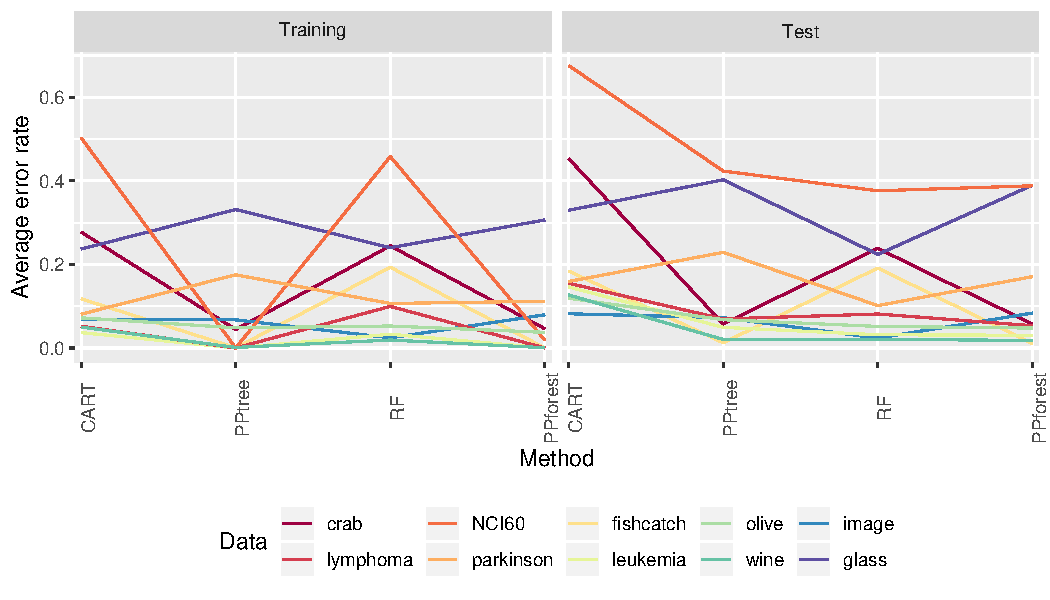
\includegraphics[width=\maxwidth]{figure/parbench-1} 

\end{knitrout}
\caption{Benchmark data results shown graphically. PPF performs consistently well across most of the data sets. \label{parallel}}
\end{figure}



\section{Diagnostics comparison}\label{options}

The diagnostics computed by PPF (Section \ref{PPFsec}) and RF are compared for the lymphoma data, which helps to understand why and how PPF outperforms RF with this data.

\subsection{Variable importance}

Figure \ref{globalimp} illustrates how the variable importance differs, using the lymphoma data. PPF outperformed RF for this data. There are three groups, and it is a high-dimension, low sample size data set. With PPF, the PDA index is used, and the 60\% of variables are available at each node. The number of trees used is the same as the RF default. Only the top ten most important variables are shown. There are some common on both lists and a some differences. Showing just the first two variables from each list is sufficient to illustrate the different type of boundaries induced by the classifiers. The two ways of computing importance in PPF do produce a different hierarchy of variables. With the global average importance, Gene35 and Gene50 are the top two, and these distinguish the small group FL best. With the global importance, Gene35 and Gene44 are featured, and together these find a big gap between DLBCL and the other two groups. PPF is utilizing the association between variables to classify groups, as would be expected.




\begin{figure}[!ht]
\begin{center}
\begin{knitrout}
\definecolor{shadecolor}{rgb}{0.969, 0.969, 0.969}\color{fgcolor}
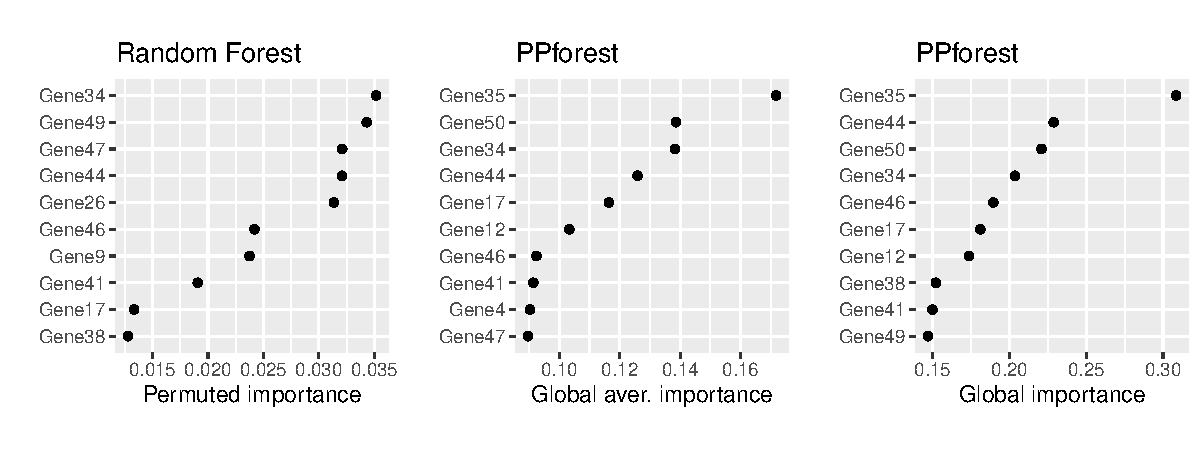
\includegraphics[width=\maxwidth]{figure/globalimpoe-1} 

\end{knitrout}
\begin{knitrout}
\definecolor{shadecolor}{rgb}{0.969, 0.969, 0.969}\color{fgcolor}
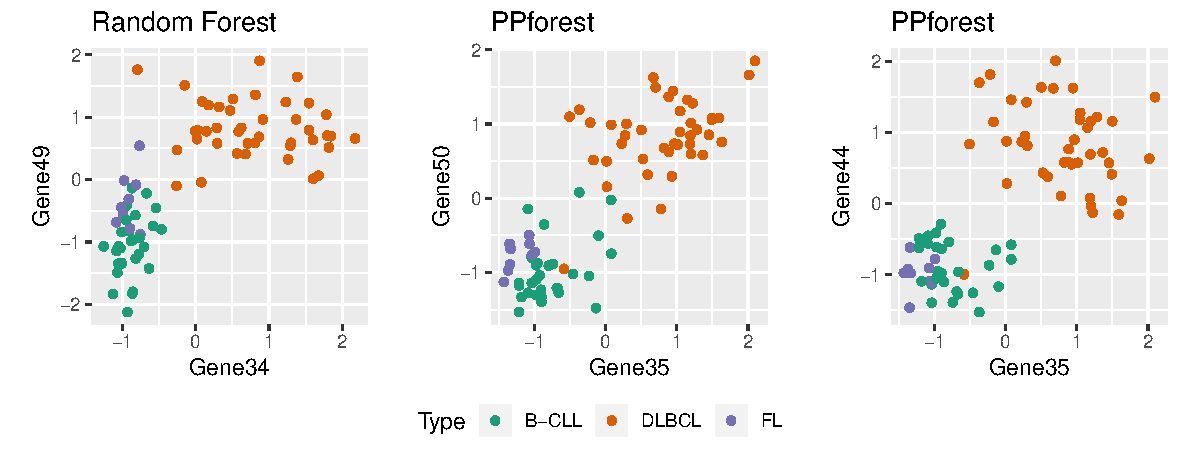
\includegraphics[width=\maxwidth]{figure/globalimpoevars-1} 

\end{knitrout}
\caption{Comparison of importance measures for the lymphoma data, where PPF outperformed RF. Top row shows the top 10 variables by each method, with two ways of calculating with PPF. Bottom row shows the top two variables from each, which illustrates the difference between methods. PPF is detecting differences between groups when there is association between variables. Using the global average importance (middle), Gene35 and Gene50 better distinguish group FL. Using the global importance, Gene35 and Gene44 find a big gap between group DLBCL and the other two. \label{globalimp}}
\end{center}
\end{figure}

\begin{figure}
\centering

\begin{knitrout}
\definecolor{shadecolor}{rgb}{0.969, 0.969, 0.969}\color{fgcolor}
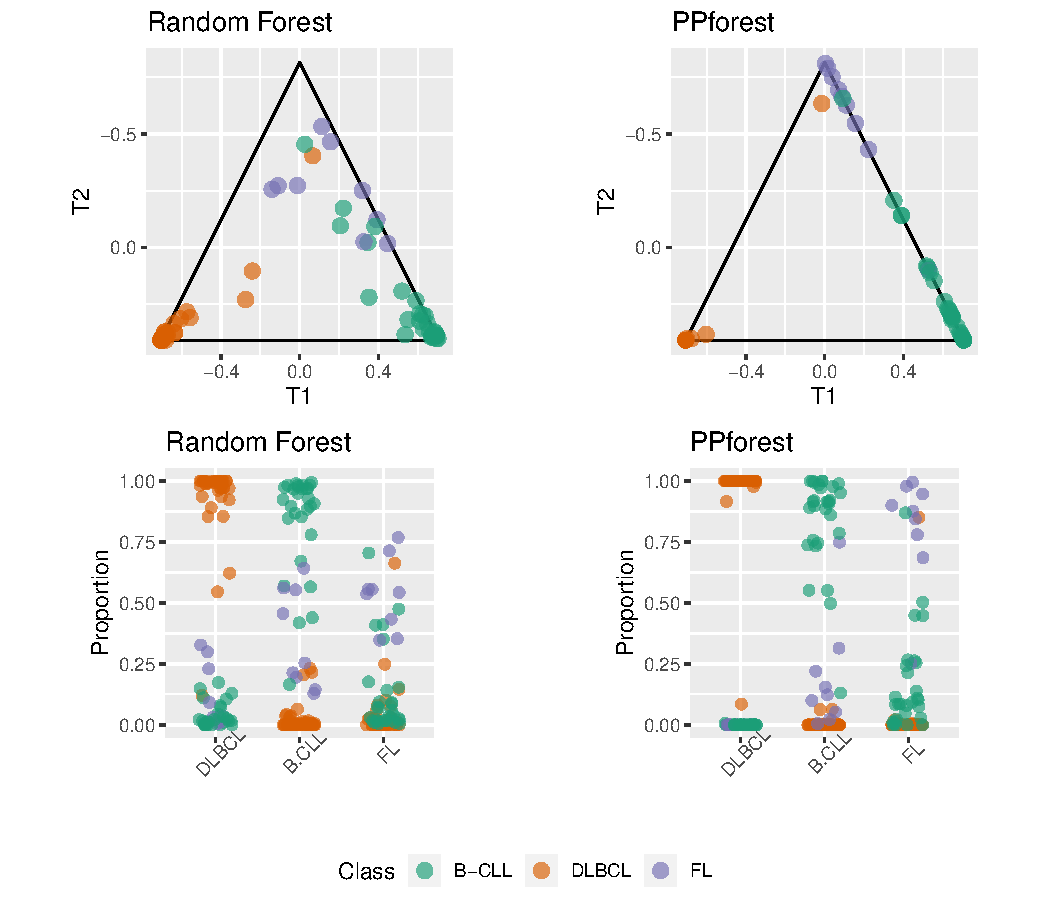
\includegraphics[width=\maxwidth]{figure/side-1} 

\end{knitrout}
\caption{Comparison of the out-of-bag vote  matrix for the three groups of the lymphoma data, returned by RF and PPF: (top) ternary plot, (bottom) side-by-side jittered dotplots. This illustrates the difference between methods. PPF votes more decisively for most cases, than RF. Especially this is true for the DLCBL class, where all but one are almost always predicted to the true class.}
\label{voteplots}
\end{figure}

\subsection{Vote matrix}

Figure \ref{voteplots} shows the vote matrices returned by PPF and RF for three classes of the lymphoma data. It is represented in two ways: as a ternary plot and as a side-by-side jittered  dotplot. The vote matrix has three columns corresponding to the proportion of times the case was predicted to be class B-CLL, DLBCL or FL, and thus is constrained to lie in a 2D triangle in 3D space. A ternary diagram is created using a helmert transformation of the vote matrix to capture the 2D subspace. The way to read it is: points near the vertex are clearly predicted to be one class, points along an edge are confused between two classes, and points in the middle are confused between the three classes. PPF provides more distinct classification of observations than RF, because the points are more concentrated in the vertices, and along one edge.

The side-by-side jittered dotplot is an alternative representation that readily can be used for any number of classes. The proportion each case is classified to a group is displayed vertically along a horizontal axis representing the categorical class variable. Points are jittered a little horizontally to better see the distribution of proportions, and colour represents the true class. Points concentrated at the top part indicate cases that are clearly grouped into a class, and if the colour matches the true class then these are correct classifications. The message is similar to the ternary diagram: DLBCL is much more clearly distinguished by PPF, and FL is actually distinguishable from B-CLL by PPF but confused by RF.


\subsection{Proximity}

\begin{figure}[!ht]
\centering
\begin{knitrout}
\definecolor{shadecolor}{rgb}{0.969, 0.969, 0.969}\color{fgcolor}
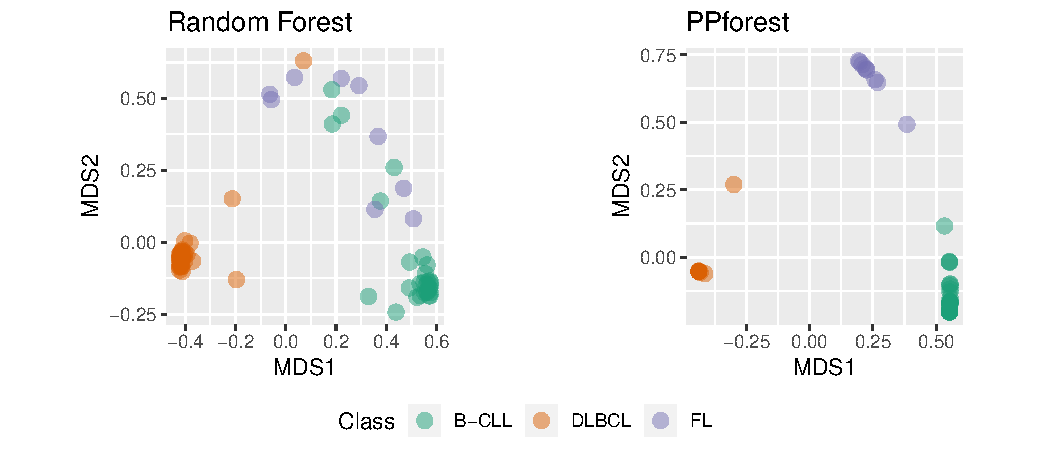
\includegraphics[width=\maxwidth]{figure/mds-1} 

\end{knitrout}
\caption{Examining similarity between cases, using pairwise plots of multidimensional scaling on the proximity matrix from RF and PPF fits of the lymphoma data. It can be seen that most cases are grouped closely with their class in PPF while in RF FL and B-CLL are mixed. \label{prox1}}
\end{figure}

Figure \ref{prox1} shows multidimensional scaling plots of the proximity matrix produced by PPF and RF classification of the lymphoma data. PPF provides the cleaner proximities. This means that more frequently observations from the same class reside in the same terminal node of the trees making up the PPF, than those of RF.

%\newpage

\subsection{Parameter selection}

The primary parameters for PPF are mostly the same as those for RF: number of trees, and number of variables used in each node partition, with the addition of $\lambda$ when PDA is used as the index.

Figure \ref{parameters} (left) shows the effect of proportion of variables for the benchmark data comparison. The average error over 200 training/test splits is shown. For several data sets error is lower when the more variables are used. Several converge to low error rate when half the variables are included. In some cases, leukemia and NCI60, the error increases when more variables are included. These two examples are where the cases variables ratio is smaller among the benchmark data set. This suggest that in small n big p problem increase the number of variables will be not the best strategy. In Section \ref{rnaapli} we will show an example to illustrate this point.

The right plot compares the number of trees needed to optimize the OOB error for both PPF and RF on the lymphoma data. Both need around 100 trees to produce best performance.


\begin{figure}[!ht]
\centering

\end{figure}
%\newpage

\begin{figure}[!ht]
\centering
\begin{knitrout}
\definecolor{shadecolor}{rgb}{0.969, 0.969, 0.969}\color{fgcolor}
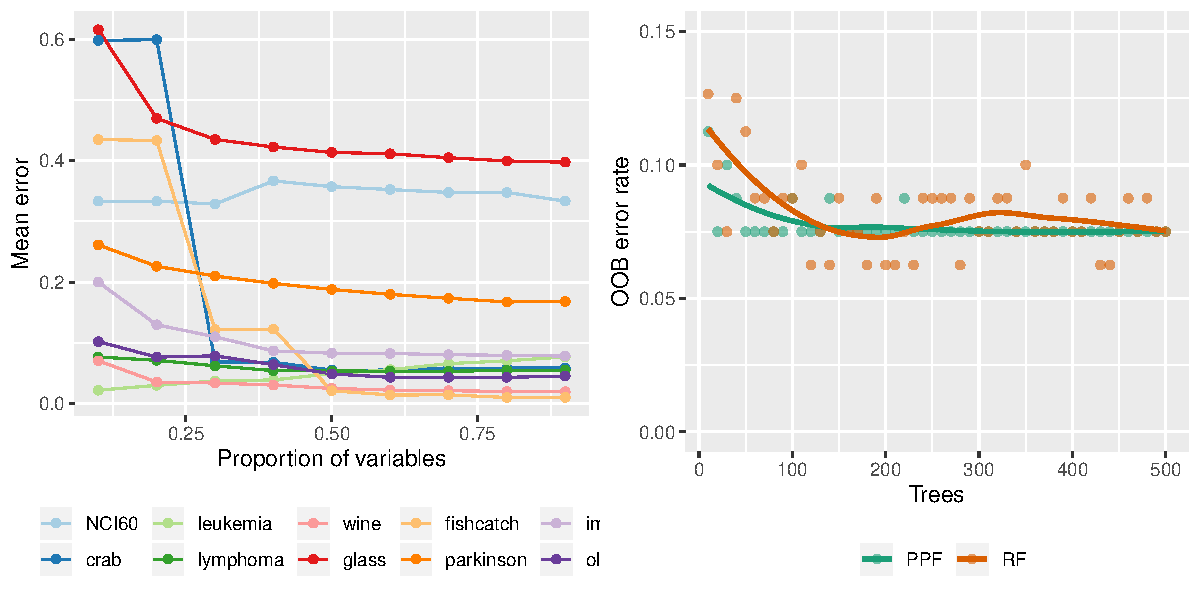
\includegraphics[width=\maxwidth]{figure/errorrate-1} 

\end{knitrout}
\caption{Illustrating model tuning using error rate reduction. The average error rate plotted against proportion of variables in all the benchmark data is shown at left. The error rate tends to be better with more variables, but it does vary substantially by data set. OOB error is plotted against number of trees (right) on the lymphoma data for both PPF and RF. PPF has the consistently lower error, but both would indicate about 100 trees is sufficient to get the best results. \label{parameters} }
\end{figure}


\section{Application: RNA-seq gene expression}\label{rnaapli}

We applied the proposed method to analyze an RNA-seq gene expression data set. The data are high-dimensional, with the number of observations, $n$ is very small relative to the number of features, $p$. Traditional classification methods like linear discriminant analysis or logistic regression cannot be applied directly in this context. PPforest can be applied for small $n$ big $p$ problem using PDA index. 

There are four genotypes of maize, two inbred genotypes (B73 and Mo17) and its reciprocal hybrids (B73xMo17 and Mo17xB7), with just four replicates of each. The details of the experiment are described in \cite{paschold2012}. A subset of 1078 genes are flagged as important for understanding the so-called gene heterosis, in at least one of the two hybrids. In plant breeding, heterosis appears when the hybrid is deferentially expressed with respect to its parents. 

We set up the classification problem as in \cite{datta2014statistical}, where the response variable is the genotype (four classes, B73, Mo17, B73xMo17 and Mo17xB7) and the feature variables are the expression of the 1078 genes. The goal is to identify important genes to distinguish among genotypes. The subset is formed with genes that are already found to be relevant, for distinguishing between inbred genotypes and its reciprocal hybrids, because choosing genes with smallest $p$-values can be misleading \citep{cook2007exploring}. To compare the predictive performance among different methods we will use leave-one out cross validation since we have a limited amount of data (16 observations).
 
% latex table generated in R 3.5.2 by xtable 1.8-2 package
% Sun Sep  8 06:41:32 2019
\begin{table}[ht]
\centering
\caption{Comparison of CART, PPF, PPtree, and RF results with maize RNA-seq gene exression data set. The mean of training and test error rates from leave-one-out cross validation is shown. PPF.03 performs favorably compared to the other methods. \label{res_RNA}} 
\begin{tabular}{l||c||c}
  \hline
Method & Training & Test \\ 
  \hline
CART & 0.733 & 1.000 \\ 
  PPF.4 & 0.000 & 0.062 \\ 
  PPF.03 & 0.000 & 0.000 \\ 
  PPtree & 0.000 & 0.062 \\ 
  RF & 0.000 & 0.250 \\ 
   \hline
\end{tabular}
\end{table}

\begin{figure}[!ht]
\centering
\begin{knitrout}
\definecolor{shadecolor}{rgb}{0.969, 0.969, 0.969}\color{fgcolor}
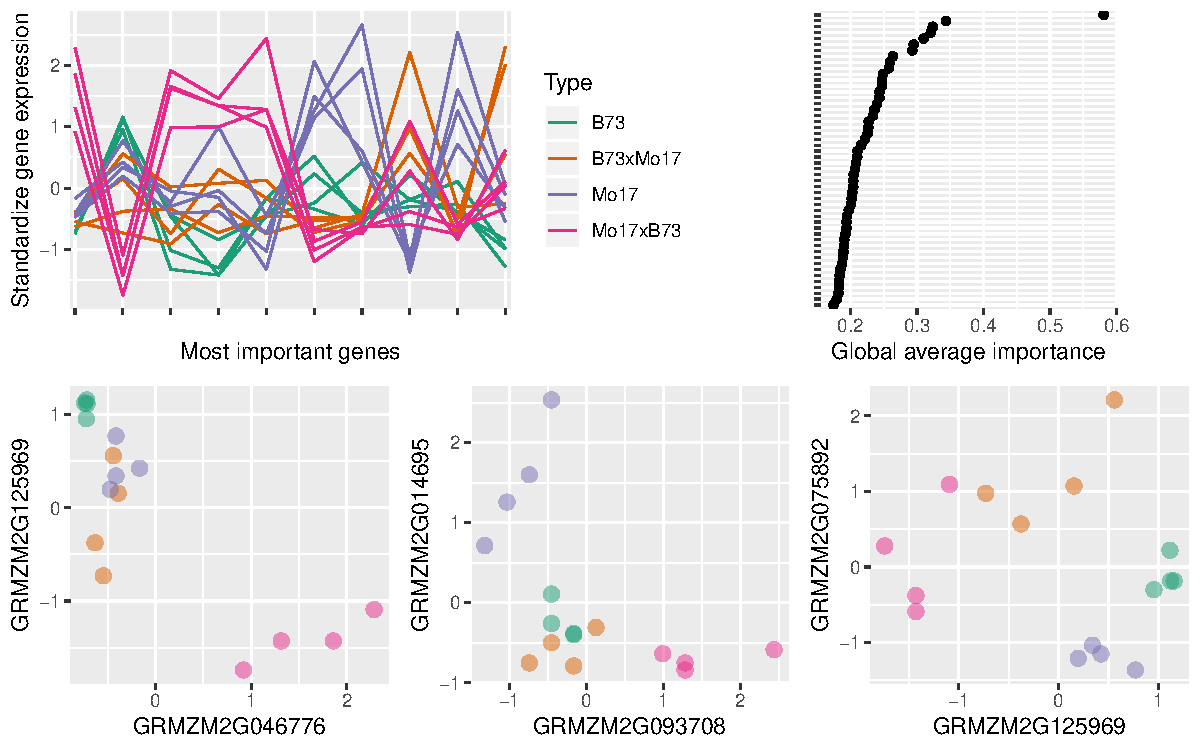
\includegraphics[width=\maxwidth]{figure/rnaseq-1} 

\end{knitrout}
\caption{Overview of the PPF results for the maize RNA-seq data. The parallel coordinate plot (top left) shows the expression values for 10 most important genes. A dotplot shows the global average importance for the top 200 genes (top right). The three scatterplots show pairs of important variables  (bottom row), indicating clear separation between classes. \label{rnacomp}}
\end{figure}




Table \ref{res_RNA} presents mean of training and test error rates from leave-one-out cross validation comparing CART, PPF, PPtree and RF. For PPF two cases are presented based on different proportions of variables considered for each node partition: PPF.4 use $40\%$ of the variables while  PPF.03 use $3\%$ of them. PPF.03, with 32 variables in each node partition, is comparable with default for RF. While PPF with $40\%$ of variables and PPtree results are the same in test error ($6.2\%$), PPF performance is better  when a smaller proportion of variables ($3\%$) is used ( $0\%$ of test error). RF presents a test error of $25\%$ using the same number of variables than PPF.03.

Figure \ref{rnacomp} shows the most important genes analysed based on global average importance measure for the best model (PPF.03). The importance measure is clearly bigger for one gene (GRMZM2G046776) and there is a breaking point in the importance measure for the first seven genes. The parallel coordinate plot shows the expression values for the top 10 variables, ordered from left to right. In the left scatterplot, of first two important variables, Mo17xB73 can be clearly separated from the other genotypes. The other scatterplots show various separations between the groups. 

With 1078 variables and only 16 observations, one might be suspicious about the results. To check this, the analysis was re-computed several times with permuted class labels, where the class label is randomly re-assigned to a different sample. This removes any real class structure, while keeping the multivariate distribution of the expression values fixed. The results showed no important variables, and little separation between classes. The results from PPF are substantially better.

\section{Discussion}\label{discpp1}

This article has presented a new ensemble method (PPF) for classification problems, that is built on an oblique tree classifier (PPtree). PPF effectively uses linear combinations of variables, incorporating the correlation between variables to build better boundaries between classes. It provides a range of diagnostics for variable importance, confusion of observations between groups and proximity of observations. PPF provides consistently low error rates, and retains the interpretability afforded by tree-based algorithms.

The benchmark data study showed that PPF's predictive performance is as good, or better than, CART and PPtree, and can outperform RF for some problems. PPF performs better than RF when the classes are separated by a linear combination of variables and when the correlation between variables increases. This can be seen by comparing the variable importance diagnostics of PPF and RF, showing that different variables are combined to create the classification model.

There are several directions where the work could be extended. The two projection pursuit indexes, LDA and PDA, can be readily supplemented by other indices, or by adapting a linear SVM. For example, using a regression index could extend the approach to a continuous response. Another direction is to adapt the PPtree algorithm to allow more than $g-1$ splits. This PPtree constraint protects the single tree model from overfitting. With PPF, there is some protection against this from bagging, and we expect it would enable deeper non-linear boundaries to be constructed. Lastly, because the accuracy of each tree is collected, automatic pruning of poor performing trees is a possibility.


\section{Acknowledgements}
\label{Aknow}

This paper was written with the R packages knitr~(\cite{xie:2015}), ggplot2 (\cite{hadley:2009}) and dplyr (\cite{dplyr}), and the files to reproduce the paper and results is available at \url{https://github.com/natydasilva/PPforestpaper}.

The authors are grateful for the helpful reviews provided by the editor, associate editor and two anonymous reviewers. 


\bibliographystyle{jasa3}
\bibliography{ppforestpaperbib}

\end{document}
